\documentclass[12pt]{article}
\usepackage{sbc-template}
\usepackage{enumerate}
\usepackage{hyperref} 
\usepackage{url} 
\usepackage{tikz}
\usepackage[utf8]{inputenc}
\usepackage[brazil]{babel}
\usepackage[T1]{fontenc}
\usepackage[scaled=0.85]{beramono}
%\usepackage[font=small,labelfont=bf,tableposition=top]{caption}
\usepackage{csquotes}
\usepackage{listings}
\usepackage{color}
\usepackage{amsmath}
\usepackage{graphicx}
\usepackage{changepage}
%\usepackage[table,xcdraw]{xcolor}
\renewcommand\lstlistingname{C\'odigo}
\setlength\parindent{20pt}

\usetikzlibrary{decorations.pathreplacing,calc}
\newcommand{\tikzmark}[1]{\tikz[overlay,remember picture] \node (#1) {};}

\newcommand\numberthis{\addtocounter{equation}{1}\tag{\theequation}}

\newcommand*{\AddNote}[4]{%
    \begin{tikzpicture}[overlay, remember picture]
        \draw [decoration={brace,amplitude=0.4em},decorate,black]
            ($(#3)!([yshift=1.5ex]#1)!($(#3)-(0,1)$)$) --  
            ($(#3)!(#2)!($(#3)-(0,1)$)$)
                node [align=center, text width=2.5cm, pos=0.5, anchor=west] {#4};
    \end{tikzpicture}
}%
     
\sloppy

%titulo
\title{Relatório Técnico Sobre uma Ferramenta para Algoritmos Genéticos - Parte 2}
%autor
\author{Vinicius Bruch Zuchi\inst{1} }

\address{Departamento de Ciência da Computação -- Universidade do Estado de Santa Catarina\\
  Centro de Ciências Tecnológicas -- Caixa Postal 15.064 -- Joinville -- SC -- Brasil
  \email{vinicius.b.zuchi@gmail.com}
}

\renewcommand\lstlistingname{C\'odigo}

\begin{document} 
\maketitle

\section{Introdução}

No trabalho anterior, foi introduzida uma ferramenta desenvolvida para a solução de 
diversos problemas diferentes utilizando algoritmos genéticos. Naquela primeira parte, 
as funcionalidades fundamentais foram desenvolvidas para que a ferramenta tivesse a 
capacidade de ser configurável e que permitisse a modelagem dos problemas listados. 

As seguintes funcionalidades foram desenvolvidas na primeira parte:
\begin{itemize}
    \item Interpretador de um arquivo de configuração, com diversos parâmetros 
        configuráveis, os quais são: tipo da codificação do indivíduo (podendo ser 
        binária, inteira, inteira permutável ou real), tamanho da população, tamanho do 
        indivíduo, limites inferior e superior para codificações não binárias, rotinas de 
        seleção, mutação e \textit{crossover} a serem utilizadas;
    \item Rotinas de seleção: roleta e torneio;
    \item Rotinas de crossover: blx, pmx, crossover uniforme e crossover de 1 ponto;
    \item Algoritmos de mutação: bit flip, swap position, delta mutation, gaussian mutation;
    \item Integração das partes do algoritmo evolutivo;
    \item Geração do gráfico de convergência
\end{itemize}

\vspace{1cm}

Mesmo que o Algoritmo Evolutivo estivesse funcionando com as funcionalidades desenvolvidas 
na primeira parte, ainda estava faltando algo que poderia ser problemático para problemas 
mais complexos: o controle da pressão seletiva e da variabilidade genética. 

O controle da pressão seletiva e da variabilidade genética são passos importantes pois 
permite que os indivíduos permaneçam mais espalhados pelo espaço de busca, e evita a 
convergência prematura, que pode em consequência fazer com que a população fique presa 
em um máximo ou mínimo local.

Para resolver esse problemas, vários algoritmos e estratégias para o controle da variabilidade 
e pressão seletiva foram implementados. Abaixo segue os algoritmos que foram implementados 
para esta segunda parte:
\begin{itemize}
    \item Escalonamento linear;
    \item Generation gap;
    \item Fitness sharing;
    \item Fator de crowding
\end{itemize}

\vspace{1cm}

Além desses algoritmos listados acima, outras funcionalidades adicionais também foram implementadas 
nesta segunda parte, estas incluem: 
\begin{itemize}
    \item Geração do gráfico da variabilidade genética;
    \item Adição de parâmetros no arquivo de configuração;
    \item Suporte a mais de uma execução do AG por execução do programa, ao final de todas as 
        execuções, são tirados dados estatísticos, como a média dos melhores, media da media, e 
        média da variabilidade de cada geração, além disso há também os melhores fitness de cada 
        execução e em qual geração o ótimo foi encontrado.
\end{itemize}

\vspace{1cm}

\section{Estratégia Para Controle da Pressão Seletiva}

Nesta seção serão discutidas as estratégias implementadas para o controle da pressão seletiva e da 
variabilidade genética e quais foram os procedimentos para fazê-las. Para todas as estratégias, há 
um valor booleano correspondente a cada uma delas no arquivo de configuração da ferramenta que 
permite a ativação e desativação de cada uma.

\subsection{Escalonamento Linear}

Como o nome sugere, o escalonamento linear realiza um escalonamento no fitness de toda a população, 
fazendo um ajuste em sua escala e deixando o valor máximo escalonado igual ao valor médio escalonado 
multiplicado por uma constante C.

Para implementar essa estratégia, foram simplesmente utilizadas as fórmulas do 
escalonamento linear, e no método de seleção, caso o escalonamento linear esteja ativado, 
um array com os fitness escalonados são utilizados no lugar dos fitness crú.

\begin{figure}[h!]
    \centering
    \begin{minipage}{0.47\textwidth}
        \centering
        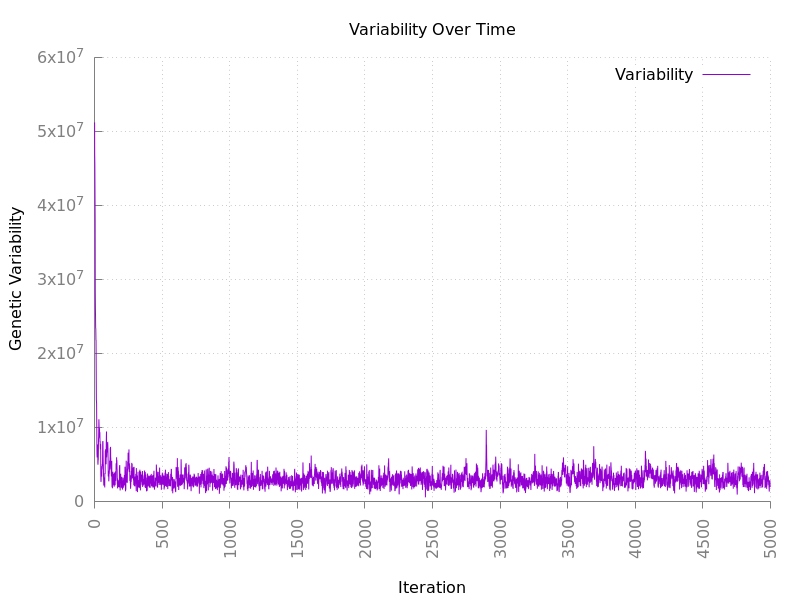
\includegraphics[width=\textwidth]{pictures/queensvarscalingoff}
        \caption{Problema das N Rainhas sem Escalonamento Linear}
        \label{f310}
    \end{minipage}
    \begin{minipage}{0.47\textwidth}
        \centering
        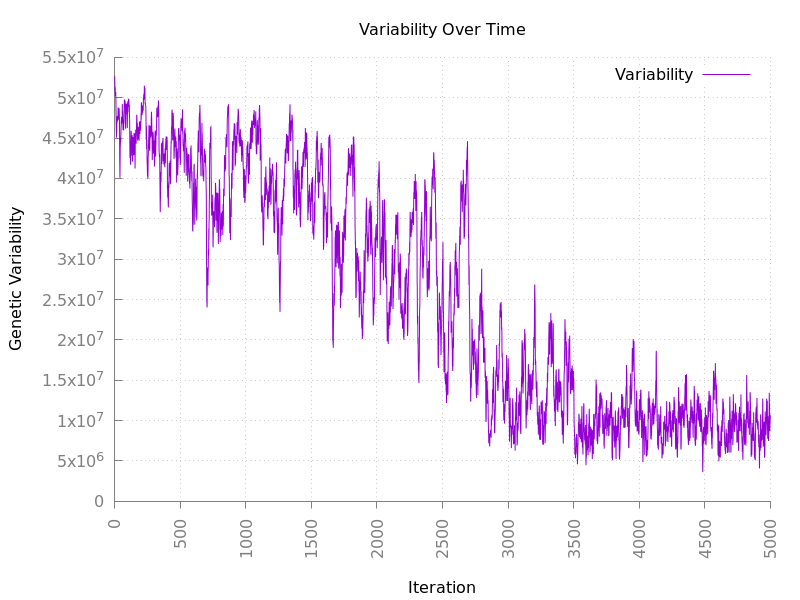
\includegraphics[width=\textwidth]{pictures/64queensvariabilityscalingon}
        \caption{Problema das N Rainhas com Escalonamento Linear}
        \label{linscaling}
    \end{minipage}
\end{figure}

Na figura~\ref{linscaling}, apesar de ter uma alta oscilação, pode-se perceber uma 
diferença no decaimento da variabilidade genética.

\subsection{Generation Gap}

O generation gap utiliza o modelo populacional de estado estável, onde os novos 
indivíduos substituem somente uma parcela da população antiga, desacelerando a velocidade 
da evolução. 

Para implementar essa estratégia, foi utilizada uma porcentagem que aumenta gradualmente 
entre 20\% e 90\% para estabelecer o tamanho da nova população gerada. Após calcular a 
porcentagem, a próxima parte é selecionar indivíduos aleatórios da população antiga para 
serem substituídos, garantido que nenhuma posição seja escolhida duas vezes.

\begin{figure}[h!]
    \centering
    \begin{minipage}{0.47\textwidth}
        \centering
        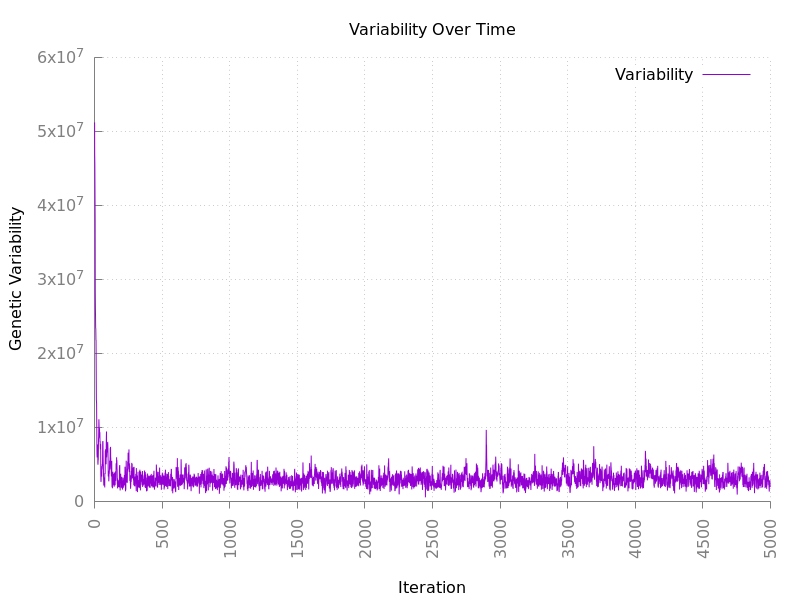
\includegraphics[width=\textwidth]{pictures/queensvarscalingoff}
        \caption{Problema das N Rainhas sem Generation Gap}
        \label{f310}
    \end{minipage}
    \begin{minipage}{0.47\textwidth}
        \centering
        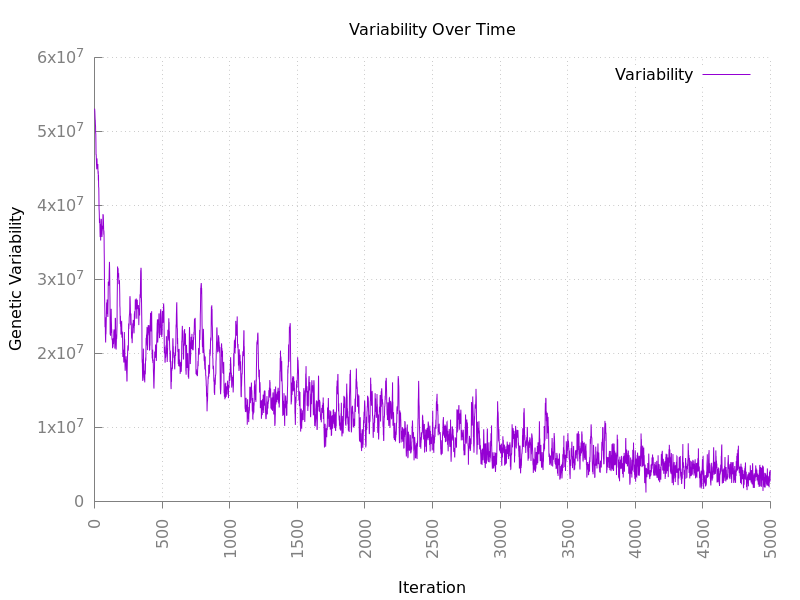
\includegraphics[width=\textwidth]{pictures/64queensvariabilitygengap}
        \caption{Problema das N Rainhas com Generation Gap}
        \label{gengap}
    \end{minipage}
\end{figure}

Comparando a figura~\ref{gengap} com a figura~\ref{linscaling}, pode-se ver que o 
generation gap obteve um sucesso muito maior em tratar a variabilidade, o decaimento 
é mais gradual e não sofre de grandes oscilações.

\subsection{Fitness Sharing}

O fitness sharing utiliza o conceito de nichos para controlar o crescimento indiscriminado 
de uma sub-população, utilizando a ideia de que indivíduos no mesmo nicho precisam 
compartilhar os recursos com outros indivíduos que pertençam ao mesmo nico.

Ou seja, quanto mais indivíduos que possuam o fitness semelhante, menor esse fitness 
ficará, desencorajando a convergência prematura de uma sub-população.

\begin{figure}[h!]
    \centering
    \begin{minipage}{0.47\textwidth}
        \centering
        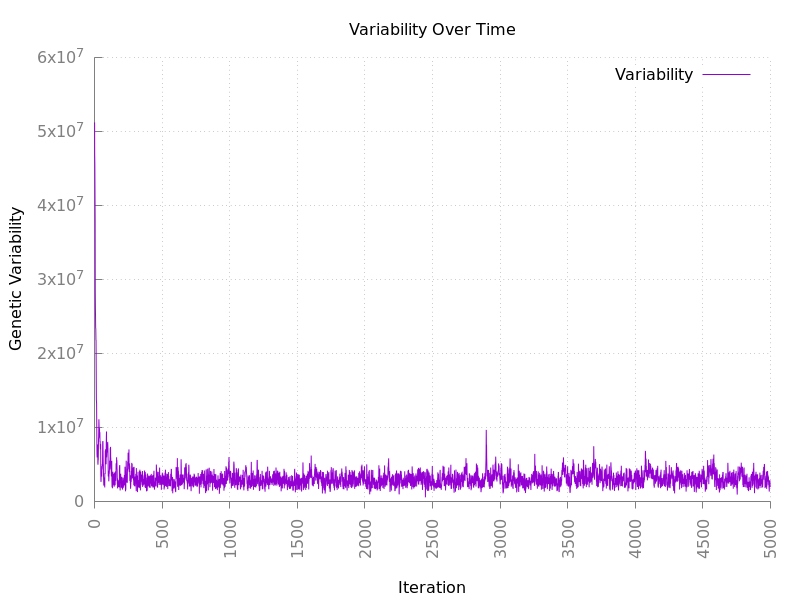
\includegraphics[width=\textwidth]{pictures/queensvarscalingoff}
        \caption{Problema das N Rainhas sem Fitness Sharing}
        \label{f310}
    \end{minipage}
    \begin{minipage}{0.47\textwidth}
        \centering
        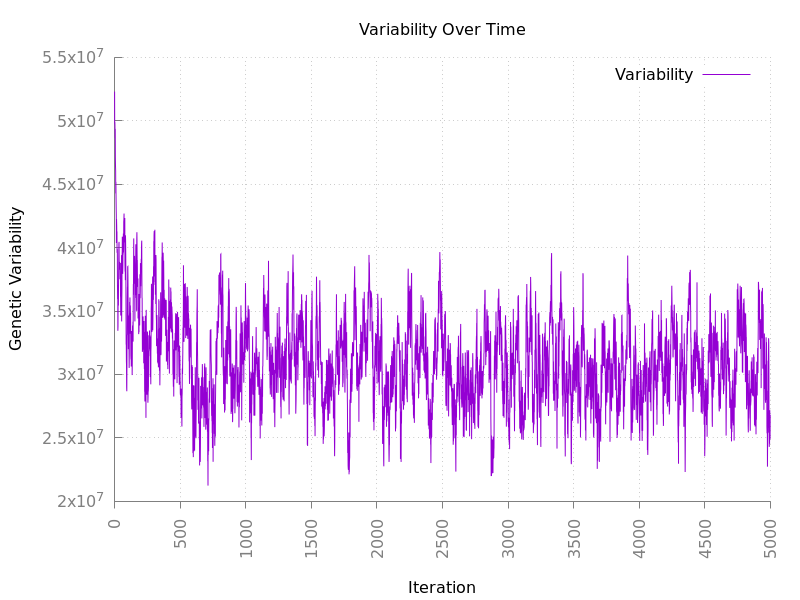
\includegraphics[width=\textwidth]{pictures/64queensvariabilitysharing}
        \caption{Problema das N Rainhas com Fitness Sharing}
        \label{sharing}
    \end{minipage}
\end{figure}

Dentre todas as estratégias de controle da variabilidade, o fitness sharing, tendo o seu 
exemplo na figura~\ref{sharing}, é o que menos demonstrou decaimento na variabilidade 
genética, isso provavelmente devido ao fato de que é a estratégia com a maior punição 
para indivíduos semelhantes.

\subsection{Fator de Crowding}

O fator de crowding também tem a intenção de diminuir a competição inter-espécies. Para 
cada indivíduo novo gerado, é selecionada uma certa quantidade (chamada de fator de 
crowding) de indivíduos aleatórios, e aquele que for mais semelhante ao novo indivíduo 
será substituído por este.

Na ferramenta, o fator de crowding que apresentou os melhores resultados foi 2. Quanto 
mais próximo de 0, o comportamento fica parecido com a utilização de nenhuma rotina, 
com uma convergência prematura. Com um fator muito alto, a variabilidade fica demasiada 
alta e a população não é capaz de evoluir.

\begin{figure}[h!]
    \centering
    \begin{minipage}{0.47\textwidth}
        \centering
        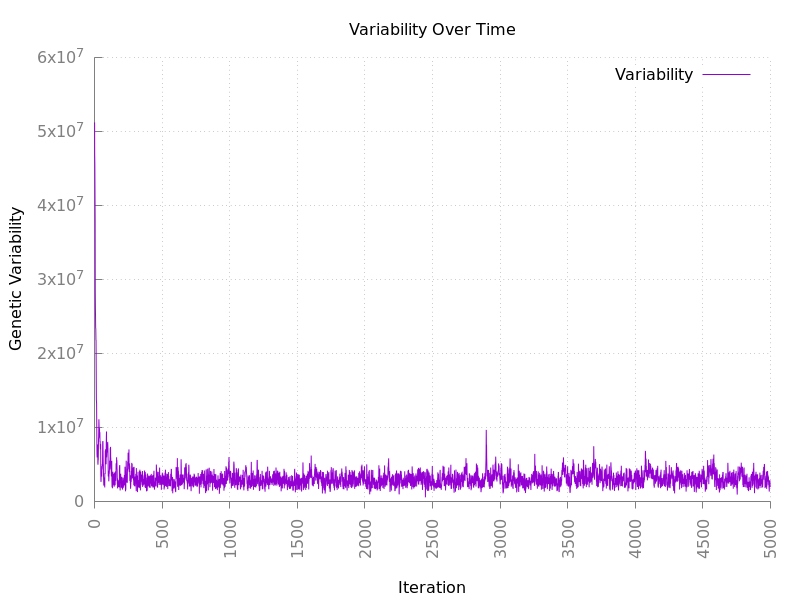
\includegraphics[width=\textwidth]{pictures/queensvarscalingoff}
        \caption{Problema das N Rainhas sem Crowding}
        \label{f310}
    \end{minipage}
    \begin{minipage}{0.47\textwidth}
        \centering
        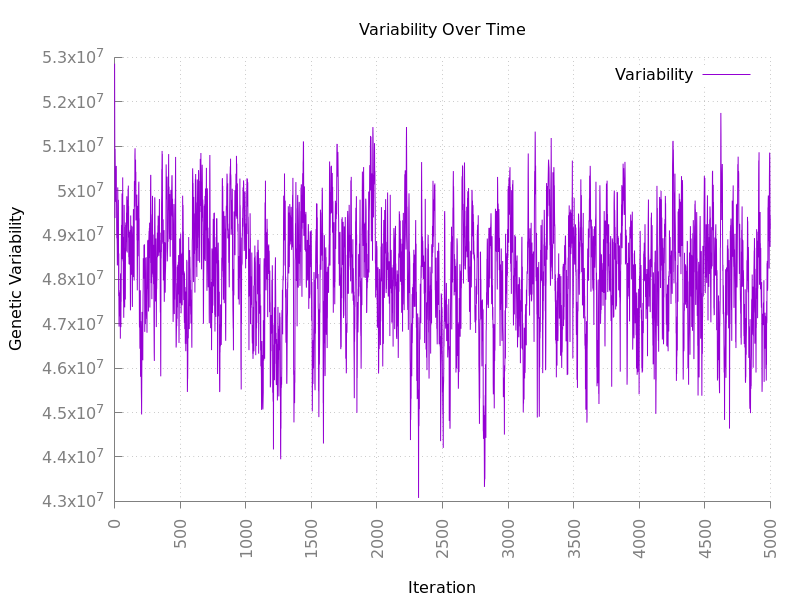
\includegraphics[width=\textwidth]{pictures/64queensvariabilitycrowding}
        \caption{Problema das N Rainhas com Crowding}
        \label{crowding}
    \end{minipage}
\end{figure}

Das estratégias de controle da variabilidade genética, o fator de crowding, representado 
pela figura~\ref{crowding} foi o que obteve o pior resultado, o gráfico dá a impressão 
de que está sendo feita uma busca aleatória.

\section{Problemas da Segunda Parte}

Nesta seção serão discutidos os problemas selecionados para fazer a segunda parte da 
ferramenta de AG.

\subsection{N Rainhas}

O problema das N rainhas consiste em dispor N rainhas em um tabuleiro de xadrez 
$N \times N$ de forma que não haja nenhuma colisão entre todas as rainhas.

Como as rainhas obrigatoriamente não podem estar em uma mesma coluna ou uma mesma linha, 
a solução para a codificação foi a utilização de inteiros permutáveis com indivíduos de 
tamanho N, onde cada gene representa uma coluna e o valor do gene uma linha, desta maneira 
a codificação já restringe naturalmente a colisão em colunas e linhas.

O cálculo do fitness então se resumiu a verificar as colisões nas diagonais entre as 
rainhas, para fazer isso utilizou-se a fórmula para verificar se dois pontos estão
alinhados diagonalmente. Esta fórmula é dada por: $|x1 - x2| = |y1 - y2|$.

Para este problema utilizou-se uma população contendo 50 indivíduos, chance de crossover 
de 80\%, chance de mutação 1\%, crossover pmx, mutação de troca entre 2 posições 
aleatórias, método de seleção torneio de tamanho 2, com elitismo e generation gap 
ativados.

Foram realizadas 10 execuções para $N = 8,\ 16,\ 32,\ 64$ com 10000 iterações cada. O 
fitness foi normalizado entre 0 e 1 para facilitar análises e visualizações.

\begin{table}[]
\centering
\caption{Média e Desvio Padrão das N rainhas para N = 8, 16, 32 e 64}
\label{nqueenstable}
\begin{tabular}{|c|c|c|}
\hline
\textbf{N Rainhas} & \textbf{Media} & \textbf{Desvio Padrão} \\ \hline
8                  & 1              & 0                      \\ \hline
16                 & 1              & 0                      \\ \hline
32                 & 1              & 0                      \\ \hline
64                 & 1              & 0                      \\ \hline
\end{tabular}
\end{table}

Como se pode ver na tabela~\ref{nqueenstable}, foi possível alcançar o ótimo 100\% das 
vezes em todos os casos, abaixar a chance de mutação de 5\% para 1\% foi um ponto crucial 
para que isso fosse possível, com a chance de mutação antiga só era atingido o ótimo 
ocasionalmente para $N = 64$, com a mudança o ótimo é sempre alcançado.

\begin{figure}[h!]
    \centering
    \begin{minipage}{0.47\textwidth}
        \centering
        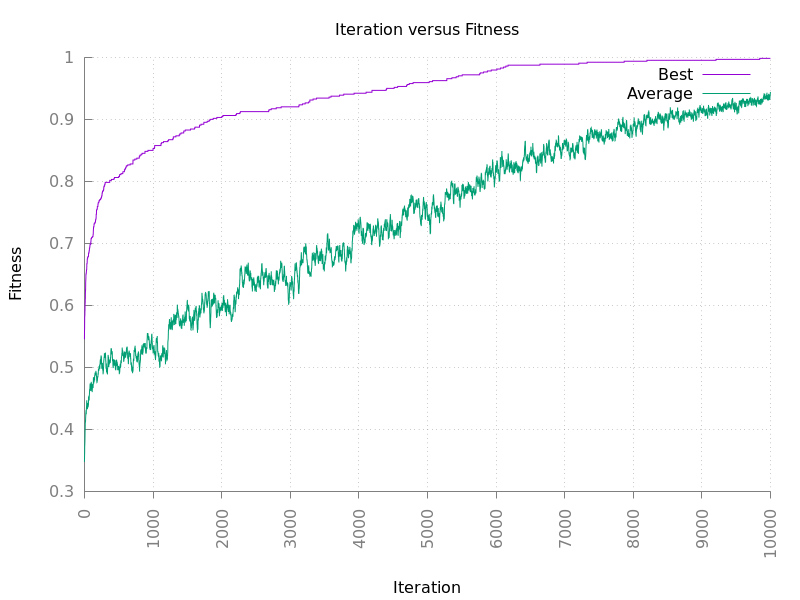
\includegraphics[width=\textwidth]{pictures/10exec64queensconvergence}
        \caption{Problema das N Rainhas sem Crowding}
        \label{10execconv}
    \end{minipage}
    \begin{minipage}{0.47\textwidth}
        \centering
        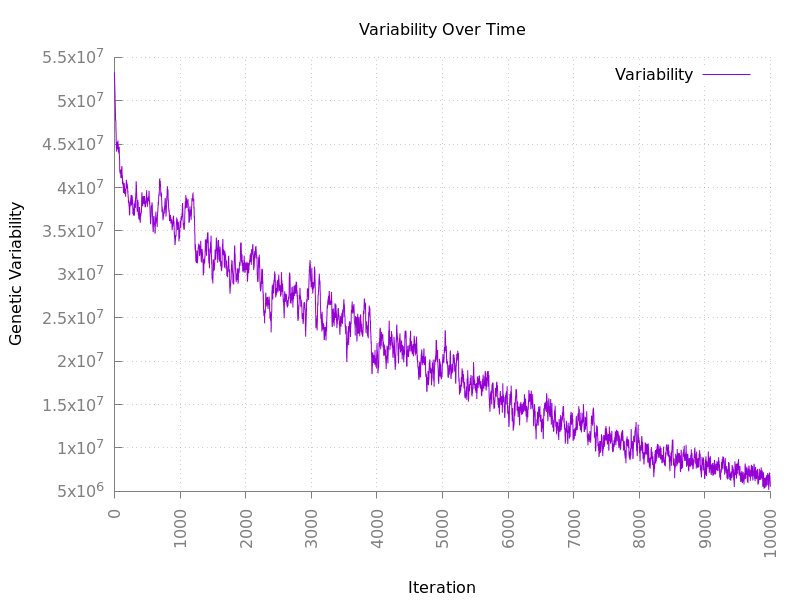
\includegraphics[width=\textwidth]{pictures/10exec64queensvariability}
        \caption{Problema das N Rainhas com Crowding}
        \label{10execvar}
    \end{minipage}
\end{figure}

Nas figuras~\ref{10execconv} e~\ref{10execvar} pode-se ver os resultados das 10 execuções 
para $N = 64$, e que as 10000 execuções foram quase insuficientes para se alcançar o 
ótimo para esse valor de $N$. O generation gap permitiu um bom controle da variabilidade 
e também a evolução gradual da população, observado pela média.

\subsection{Problema do Caminho Mínimo}

Esse problema consiste em achar um caminho mínimo por um labirinto com obstáculos, onde 
há um ponto de partida e um ponto de destino.

Para a representação do labirinto, foi utilizada uma matriz com 0's e 1's, onde o número 
1 representa as células com obstáculos. Quanto aos indivíduos, como o limite de 
movimentos era 100, foram utilizados indivíduos de tamanho 100 contendo inteiros variando 
entre 1 e 4, onde cada um desses números é então mapeado para uma das possíveis instruções, 
que são a movimentação para a esquerda e direita, para cima e para baixo.

No cálculo do fitness o movimento representado por cada indivíduo é simulado seguindo as 
instruções uma por uma, quando um movimento é impedido por um obstáculo, não se muda a 
célula da posição atual. O fitness é bonificado pela proximidade do destino, por um 
sem ou com poucas colisões e pela verificação da chegada ao destino ou não. São aplicadas 
penalidades por colisões e por caminhos repetidos do indivíduo.

Porém a modelagem desse problema não foi bem sucedida, os resultados foram longe de 
satisfatórios e por isso decidiu-se não colocar resultados nesse relatório

\subsection{Problemas Enganadores}

Os problemas enganadores conduzem a evolução da população a um caminho errôneo. Para contornar
esse problema, é necessário que os parâmetros e as rotinas utilizadas no AG estejam devidamente 
configuradas para um certo problema. 

A seguir serão mostrados os resultados obtidos com o uso da ferramenta para solucionar os problemas 
enganadores: f310, f320, f310s, f320s, d16 4 e d32 4. Para se ter um limiar, um SA também foi 
utilizado para a solução desses problemas e seus resultados foram comparados com os do GA.

No caso do GA, para todos os problemas, foi utilizada uma chance de crossover de 80\%, uma chance de 
mutação de 1\%, crossover uniforme, mutação bit flip, método de seleção torneio de tamanho 2, elitismo 
ativado e generation gap incremental com início de 20\%  de novos indivíduos até 90\%.

Para o GA, os problemas f310 e f310s, 5000 iterações foram o suficiente para chegar ao ótimo. Para os 
problemas f320 e f320, d16 4 e d32 4 foram utilizadas 100000 iterações. No caso do SA, foram utilizadas 
500000 iterações para todos os casos. Para ambos, todos os problemas foram executados 10 vezes para 
se obter a média e o desvio padrão.

\begin{table}[]
    \begin{adjustwidth}{-2cm}{}
\centering
\caption{Comparativo entre o AG e o SA para os diferentes problemas enganadores.}
\label{gasatable}
\begin{tabular}{|c|c|c|}
\hline
\textbf{F3 10}                                                                        & \textbf{AG}                             & \textbf{SA}                         \\ \hline
Taxa de Sucesso (\%)                                                                  & 100\%                                   & 0\%                                 \\ \hline
Média do Melhor Valor                                                                 & Media: 1 | Desvio Padrão: 0             & Media: 0.968 | Desvio Padrão: 0.01  \\ \hline
\begin{tabular}[c]{@{}c@{}}Número de Avaliações para\\ encontrar o ótimo\end{tabular} & Media: 1475.6 | Desvio Padrão: 221.52   & -                                   \\ \hline
\textbf{F3 20}                                                                        & \textbf{AG}                             & \textbf{SA}                         \\ \hline
Taxa de Sucesso (\%)                                                                  & 100\%                                   & 0\%                                 \\ \hline
Média do Melhor Valor                                                                 & Media: 1 | Desvio Padrão: 0             & Media: 0.892 | Desvio Padrão: 0.01  \\ \hline
\begin{tabular}[c]{@{}c@{}}Número de Avaliações para\\ encontrar o ótimo\end{tabular} & Media: 45092.1 | Desvio Padrão: 3852    & -                                   \\ \hline
\textbf{F3S 10}                                                                       & \textbf{AG}                             & \textbf{SA}                         \\ \hline
Taxa de Sucesso (\%)                                                                  & 100\%                                   & 0\%                                 \\ \hline
Média do Melhor Valor                                                                 & Media: 1 | Desvio Padrão: 0             & Media: 0.966 | Desvio Padrão: 0.007 \\ \hline
\begin{tabular}[c]{@{}c@{}}Número de Avaliações para\\ encontrar o ótimo\end{tabular} & Media: 1809.6 | Desvio Padrão: 463.1    & -                                   \\ \hline
\textbf{F3S 20}                                                                       & \textbf{AG}                             & \textbf{SA}                         \\ \hline
Taxa de Sucesso (\%)                                                                  & 100\%                                   & 0\%                                 \\ \hline
Média do Melhor Valor                                                                 & Media: 1 | Desvio Padrão: 0             & Media: 0.903 | Desvio Padrão: 0.01  \\ \hline
\begin{tabular}[c]{@{}c@{}}Número de Avaliações para\\ encontrar o ótimo\end{tabular} & Media: 21955.4 | Desvio Padrão: 3966.3  & -                                   \\ \hline
\textbf{D16 4}                                                                        & \textbf{AG}                             & \textbf{SA}                         \\ \hline
Taxa de Sucesso (\%)                                                                  & 100\%                                   & 0\%                                 \\ \hline
Média do Melhor Valor                                                                 & Media: 1 | Desvio Padrão: 0             & Media: 0.743 | Desvio Padrão: 0.01  \\ \hline
\begin{tabular}[c]{@{}c@{}}Número de Avaliações para\\ encontrar o ótimo\end{tabular} & Media: 75875.1 | Desvio Padrão: 15012.2 & -                                   \\ \hline
\textbf{D32 4}                                                                        & \textbf{AG}                             & \textbf{SA}                         \\ \hline
Taxa de Sucesso (\%)                                                                  & 0\%                                     & 0\%                                 \\ \hline
Média do Melhor Valor                                                                 & Media: 0.861 | Desvio Padrão: 0.02      & Media: 0.651 | Desvio Padrão: 0.01  \\ \hline
\begin{tabular}[c]{@{}c@{}}Número de Avaliações para\\ achar o ótimo\end{tabular}     & -                                       & -                                   \\ \hline
\end{tabular}
    \end{adjustwidth}
\end{table}

Analisando a tabela~\ref{gasatable}, pode-se observar que o SA obteve um desempenho inferior 
em todos os problemas e não foi capaz de encontrar o ótimo em nenhum dos casos, visto que 
não é um algoritmo populacional e não possui estratégias avançadas para explorar o espaço 
de busca como o GA possui.

Todos os problemas tiveram o fitness normalizado entre 0 e 1 para facilitar as comparações 
e também facilitar a visualização dos gráficos, pois todos terão a mesma referência.

\begin{figure}[h!]
    \centering
    \begin{minipage}{0.45\textwidth}
        \centering
        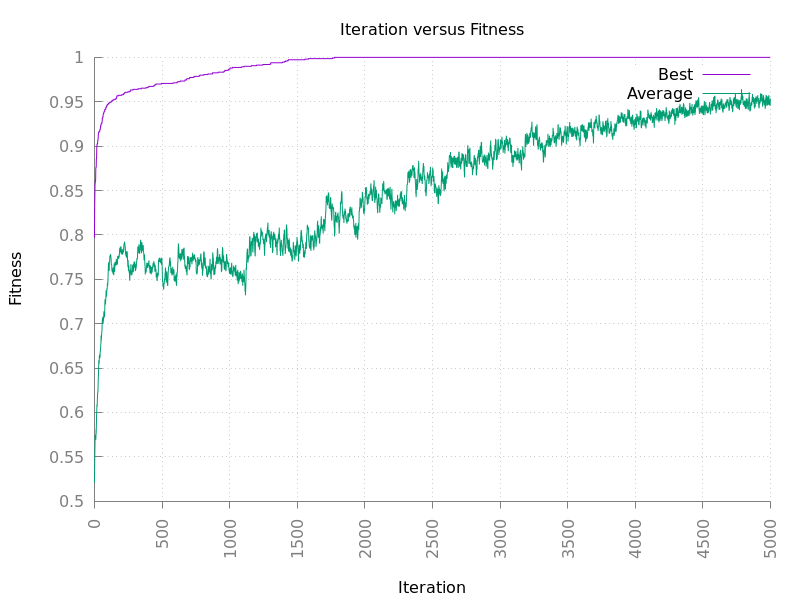
\includegraphics[width=\textwidth]{pictures/f310convergence}
        \caption{Convergência do f310 para o GA}
        \label{f310}
    \end{minipage}
    \begin{minipage}{0.45\textwidth}
        \centering
        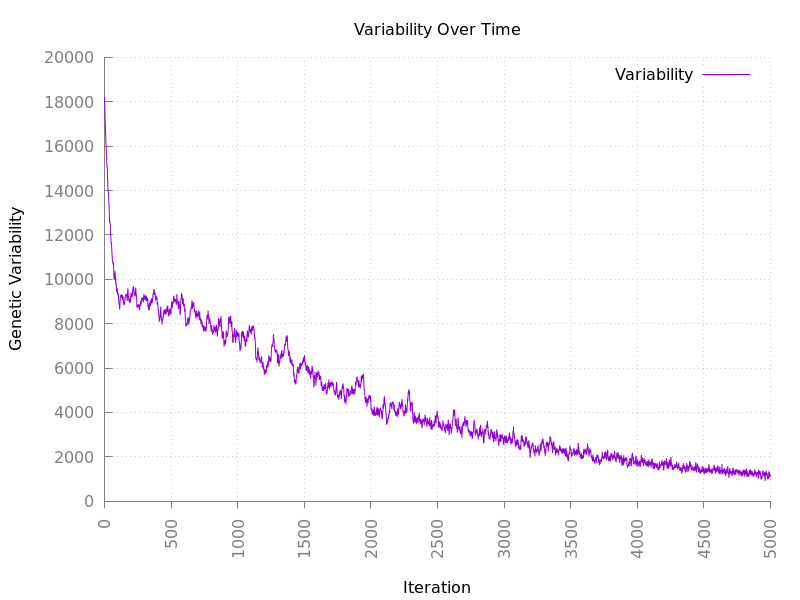
\includegraphics[width=\textwidth]{pictures/f310variability}
        \caption{Variabilidade Genética do f310}
    \end{minipage}
\end{figure}

\begin{figure}[h!]
    \centering
    \begin{minipage}{0.45\textwidth}
        \centering
        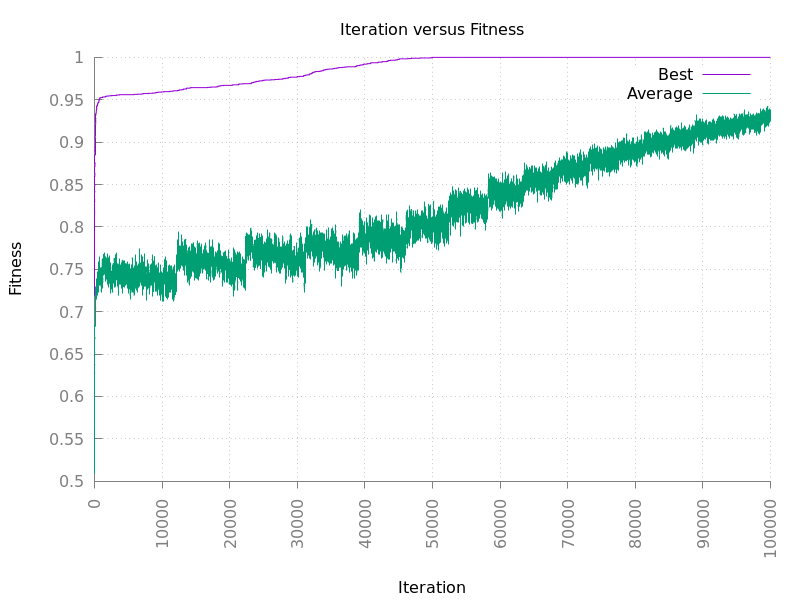
\includegraphics[width=\textwidth]{pictures/f320convergence}
        \caption{Convergência do f320 para o GA}
    \end{minipage}
    \begin{minipage}{0.45\textwidth}
        \centering
        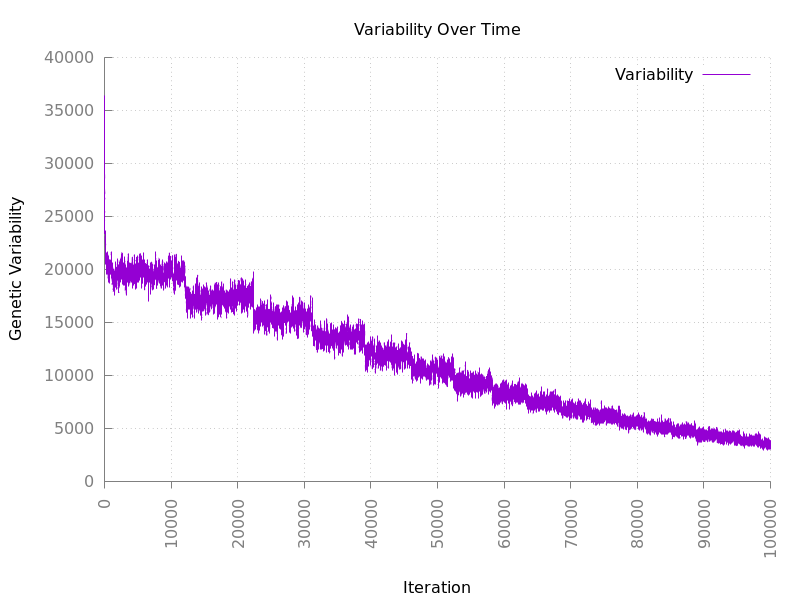
\includegraphics[width=\textwidth]{pictures/f320variability}
        \caption{Variabilidade Genética do f320}
    \end{minipage}
\end{figure}

\begin{figure}[h!]
    \centering
    \begin{minipage}{0.45\textwidth}
        \centering
        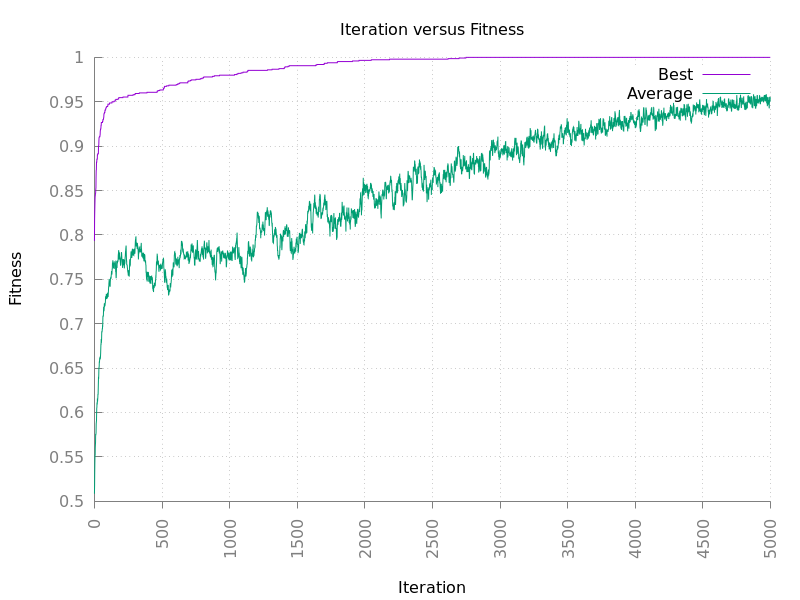
\includegraphics[width=\textwidth]{pictures/f310sconvergence}
        \caption{Convergência do f310s para o GA}
    \end{minipage}
    \begin{minipage}{0.45\textwidth}
        \centering
        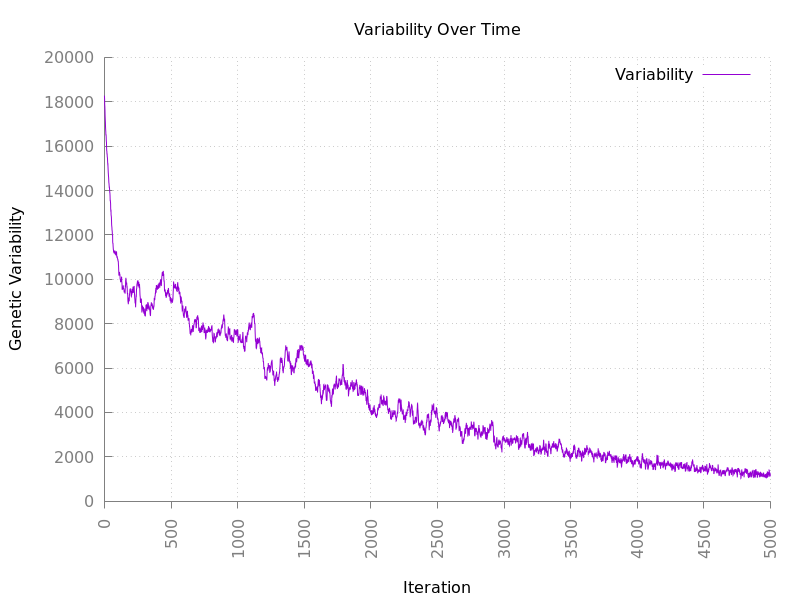
\includegraphics[width=\textwidth]{pictures/f310svariability}
        \caption{Variabilidade Genética do f310s}
    \end{minipage}
\end{figure}

\begin{figure}[h!]
    \centering
    \begin{minipage}{0.45\textwidth}
        \centering
        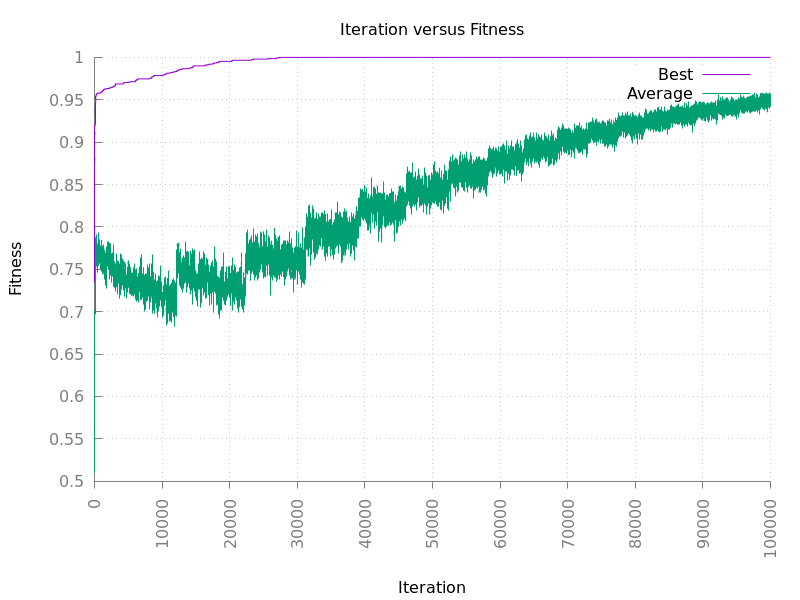
\includegraphics[width=\textwidth]{pictures/f320sconvergence}
        \caption{Convergência do f320s para o GA}
    \end{minipage}
    \begin{minipage}{0.45\textwidth}
        \centering
        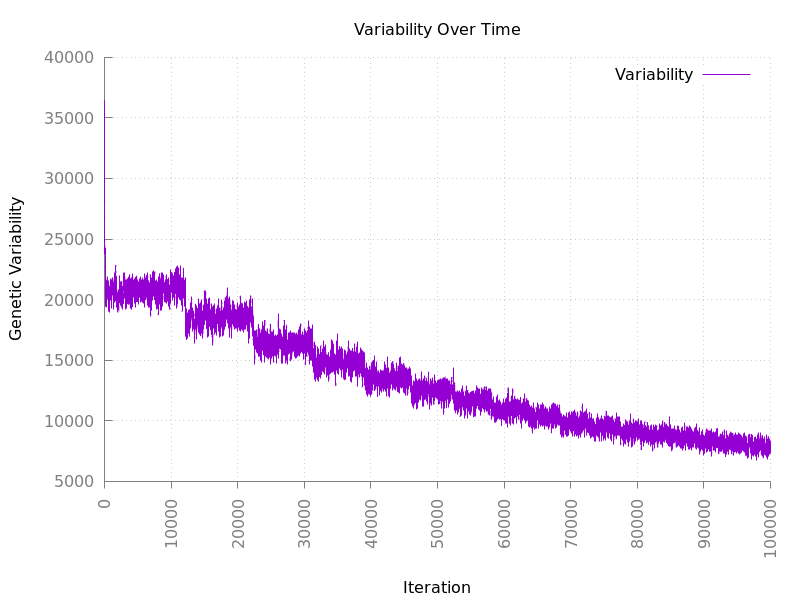
\includegraphics[width=\textwidth]{pictures/f320svariability}
        \caption{Variabilidade Genética do f320s}
    \end{minipage}
\end{figure}

\begin{figure}[h!]
    \centering
    \begin{minipage}{0.45\textwidth}
        \centering
        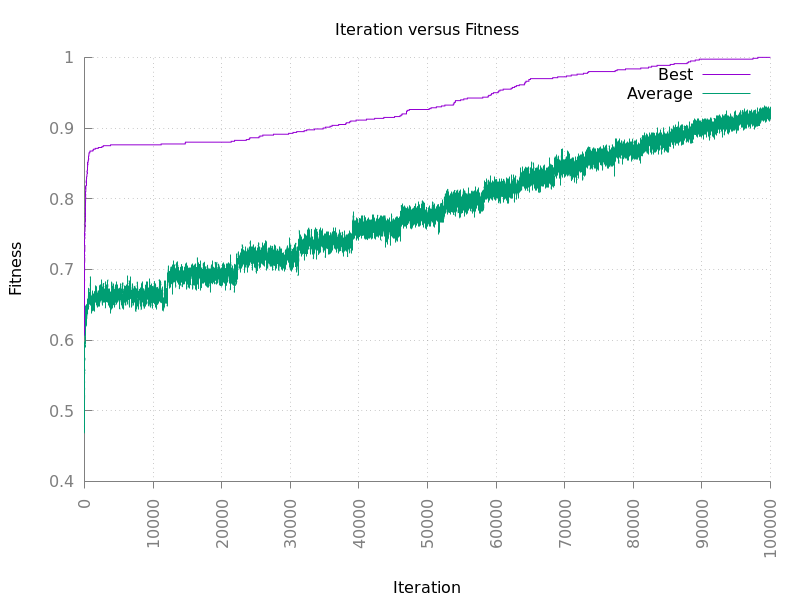
\includegraphics[width=\textwidth]{pictures/d164convergence}
        \caption{Convergência do d164 para o GA}
    \end{minipage}
    \begin{minipage}{0.45\textwidth}
        \centering
        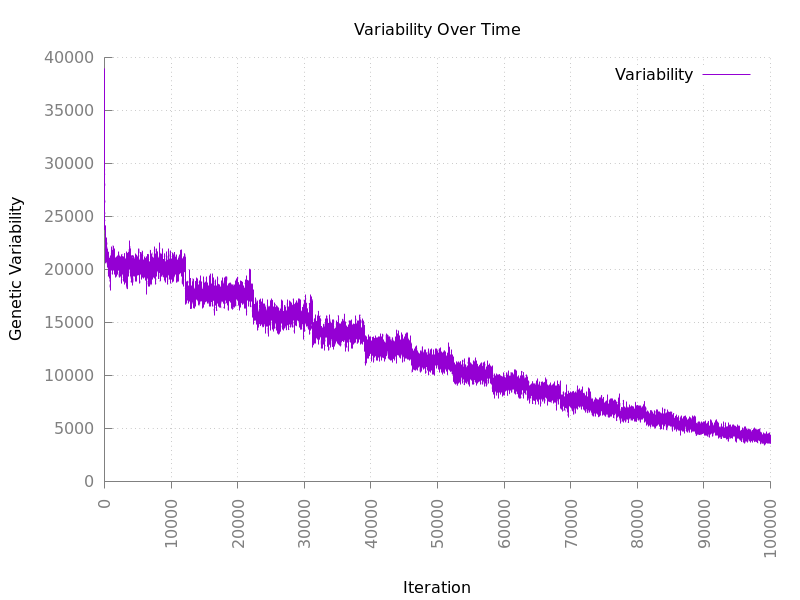
\includegraphics[width=\textwidth]{pictures/d164variability}
        \caption{Variabilidade Genética do d164}
    \end{minipage}
\end{figure}

\begin{figure}[h!]
    \centering
    \begin{minipage}{0.45\textwidth}
        \centering
        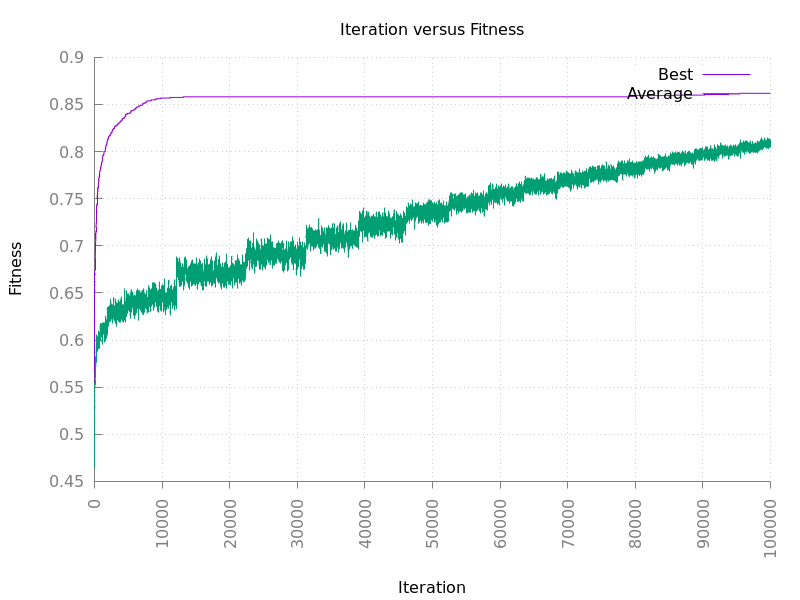
\includegraphics[width=\textwidth]{pictures/d324convergence}
        \caption{Convergência do d324 para o GA}
    \end{minipage}
    \begin{minipage}{0.45\textwidth}
        \centering
        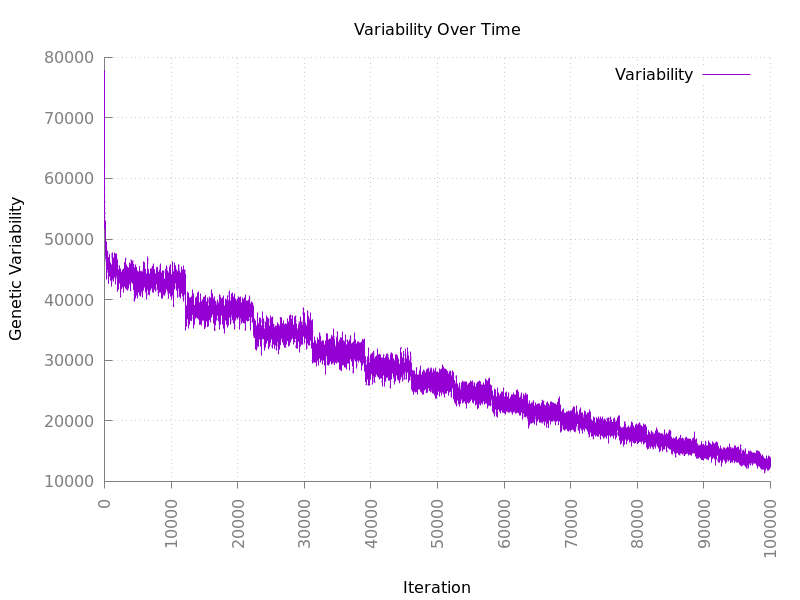
\includegraphics[width=\textwidth]{pictures/d324variability}
        \caption{Variabilidade Genética do d324}
        \label{d324}
    \end{minipage}
\end{figure}

Analisando as figuras~\ref{f310} a~\ref{d324}, percebe-se que para o GA as funções 
enganadoras tiveram um comportamento semelhante tanto na convergência do fitness 
quanto na variabilidade genética, o uso do generation gap permitiu que a variabilidade 
tivesse um decaimento gradual.

A diferença que se pode observar, além das diferentes quantidades de iterações para se 
chegar no ótimo, é a diferença de oscilação na variedade genética entre as funções 
f310 e f310s, que tiveram uma oscilação menos densa, enquanto as outras tiveram uma 
oscilação mais densa, devido a um maior espaço de busca.

\begin{figure}[h!]
    \centering
    \begin{minipage}{0.45\textwidth}
        \centering
        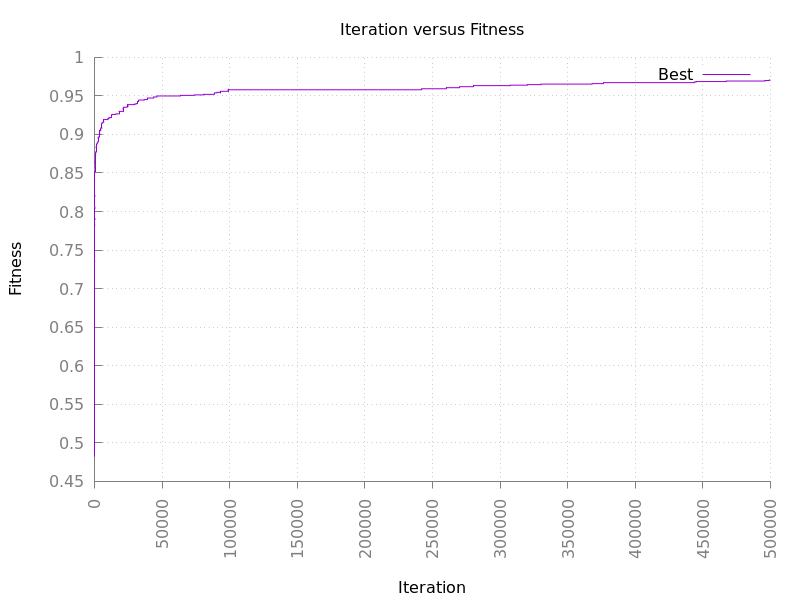
\includegraphics[width=\textwidth]{pictures/saf310}
        \caption{Convergência do f310 para o SA}
        \label{sa310}
    \end{minipage}
    \begin{minipage}{0.45\textwidth}
        \centering
        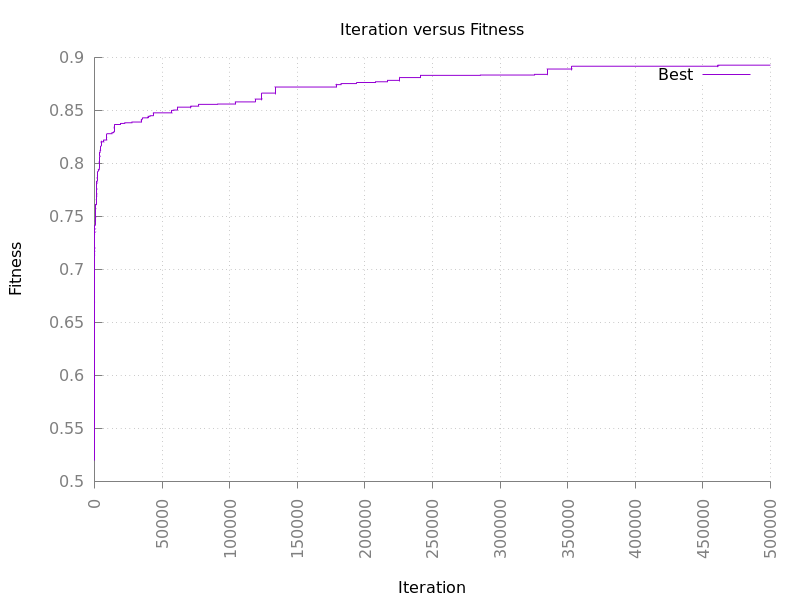
\includegraphics[width=\textwidth]{pictures/saf320}
        \caption{Convergência do f320 para o SA}
    \end{minipage}
\end{figure}

\begin{figure}[h!]
    \centering
    \begin{minipage}{0.45\textwidth}
        \centering
        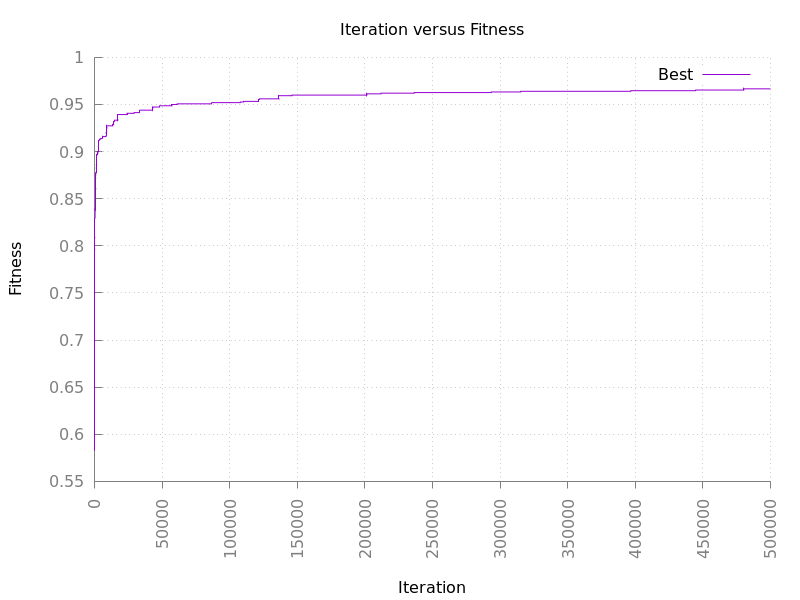
\includegraphics[width=\textwidth]{pictures/saf310s}
        \caption{Convergência do f310s para o SA}
    \end{minipage}
    \begin{minipage}{0.45\textwidth}
        \centering
        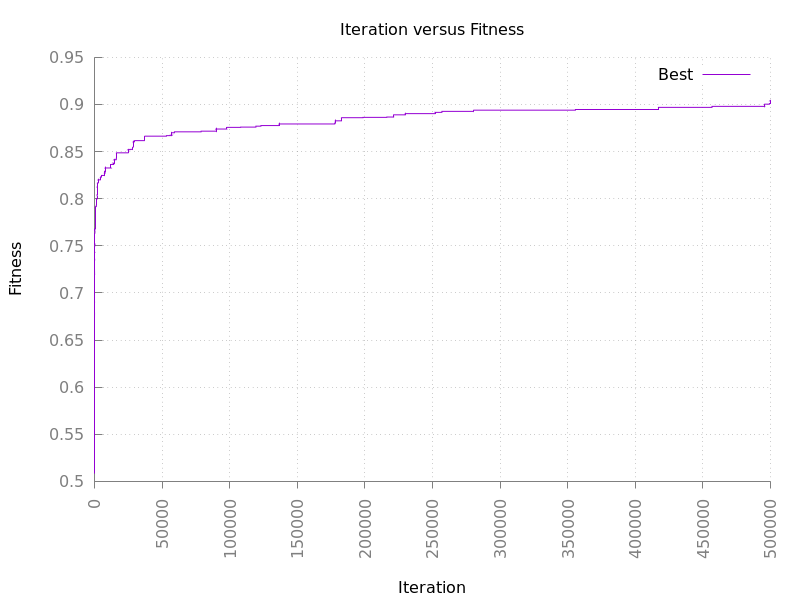
\includegraphics[width=\textwidth]{pictures/saf320s}
        \caption{Convergência do f320s para o SA}
    \end{minipage}
\end{figure}

\begin{figure}[h!]
    \centering
    \begin{minipage}{0.45\textwidth}
        \centering
        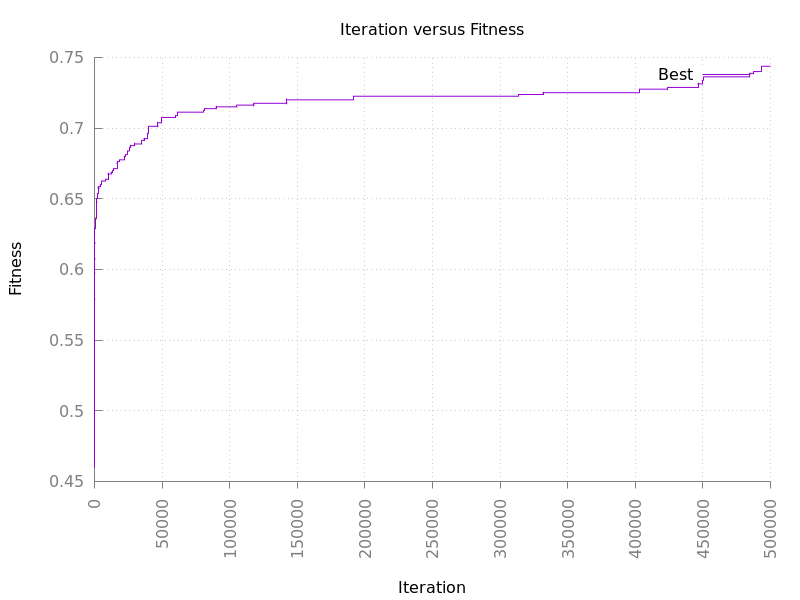
\includegraphics[width=\textwidth]{pictures/sad164}
        \caption{Convergência do d16 4 para o SA}
    \end{minipage}
    \begin{minipage}{0.45\textwidth}
        \centering
        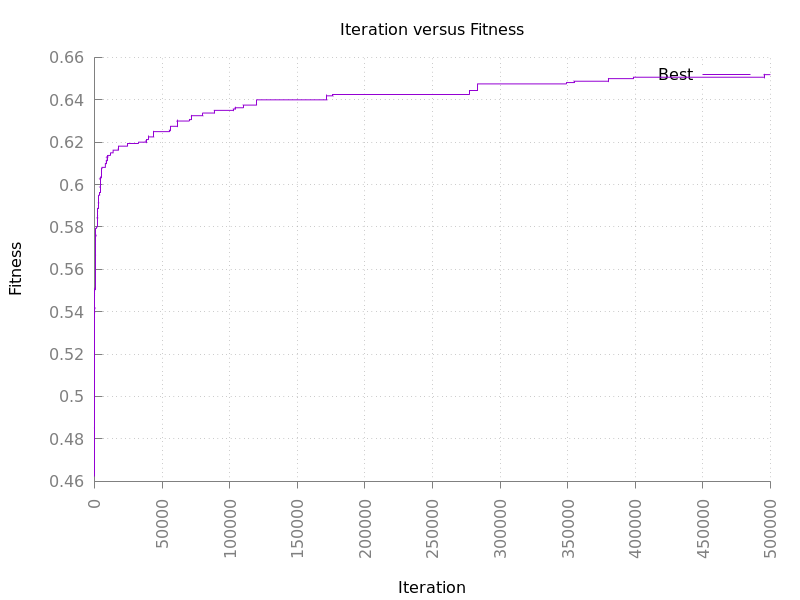
\includegraphics[width=\textwidth]{pictures/sad324}
        \caption{Convergência do d32 4 para o SA}
        \label{sa324}
    \end{minipage}
\end{figure}

Analisando as figuras~\ref{sa310} a~\ref{sa324}, pode-se observar que todas possuem um 
comportamento muito similar. O SA apesar de conseguir ter um crescimento firme até certo 
ponto, não é capaz de chegar ao ótimo pois sempre fica estagnado nos máximos locais dos 
problemas enganadores.

\section{Conclusão}

Os algoritmos evolutivos são capazes de resolver uma alta gama de problemas diferentes e 
sua implementação geralmente não requer um conhecimento profundo teórico sobre o problema 
sendo modelado.

A codificação e a concepção da função de fitness são dois passos cruciais para a resolução 
adequada do problema sendo modelado.

A utilização dos parâmetros adequados é também um passo igualmente crucial para o sucesso 
do algoritmo evolutivo, sendo interessante buscar por maneiras de se encontrar os 
parâmetros ideias sem recorrer à tentativa e erro.

Além disso, é também necessário que haja um controle na pressão seletiva da população e 
na variabilidade genética, a convergência prematura da população tem o risco de fazer 
com que esta fique presa em um máximo local, não explorando completamente o espaço de 
busca.

Modelar um problema de caminho mínimo através de um algoritmo evolutivo é algo 
extremamente difícil.

%\bibliographystyle{sbc}
%\bibliography{sbc-template}

\end{document}
